% Chapter 1

\chapter{Grundlagen} % Main chapter title

\label{Chapter2} % For referencing the chapter elsewhere, use \ref{Chapter1} 

%----------------------------------------------------------------------------------------

% Define some commands to keep the formatting separated from the content 


%----------------------------------------------------------------------------------------



Das folgende Kapitel dient dazu die in der Einleitung genannten Begriffe und Prinzipien genauer zu erläutern. Wir wollen also zunächst BPMN und die Bestandteile der Modellierungssprache genauer betrachten. Hierzu werden wir jedes Element einzeln betrachten und dadurch stück für Stück ein passendes Beispiel erstellen. Dieses Beispiel wird auch im Rest der Arbeit Relevanz finden. 
Im Anschluss wird dann die verwendete Prozessalgebra genauer betrachtet. Auch hier wollen wir jeden Bestandteil des Modells im Detail erläutern.
\section{BPMN}\label{BPMN}
Wie in der Einleitung bereits erwähnt, dient BPMN der graphischen Darstellung von Business Prozessen. In BPMN werden diese Prozesse in einzelne Aktivitäten oder Aufgaben unterteilt und dann in der richtigen Reihenfolge aufgezeichnet. Es gibt unterschiedliche Möglichkeiten Verzweigungen, Abhängigkeiten und Ähnliches zu Modellieren doch zum größten Teil basiert alles auf der korrekten Aneinanderreihung dieser Aktivitäten.
\subsection{Erste Schritte - Events und Aktivitäten}\label{Erste Schritte - Events und Aktivitäten}
Im folgenden Abschnitt schauen wir uns also die von uns verwendete Teilmenge der Modellierungssprache BPMN an. Hierzu möchten wir zunächst einen einführenden Prozess als Beispiel betrachten. Für alle möglichen Homepages und Websites von unterschiedlichen Firmen und Anbietern können Konten erstellt werden. Diese dienen zur Wiedererkennung eines Kunden oder Mitarbeiters. In diesem Abschnitt wollen wir ein BPMN-Diagramm erstellen, welches den Registrierungsprozess auf einer solchen Website darstellen könnte. Wir werden die Modellierungssprache hierzu aufteilen und jeden Bestandteil der Sprache anhand des Beispiels einzeln erläutern, sodass wir am ende dieses Abschnittes ein erstes, vollständiges Diagramm vorfinden.\\
Die von uns genutzte Teilmenge kann in einzelne Blöcke eingeteilt werden. Diese können in zwei Gruppen unterteilt werden. Die \textit{Basic Blocks} und die \textit{Flow Blocks}. Des Weiteren kann unterschieden werden zwischen \textit{Leaf Blocks} und \textit{Nonleaf Blocks}. Alle \textit{Nonleaf Blocks} bestehen aus beliebig vielen \textit{Leaf Blocks}. Es existieren genau zwei für uns relevante \textit{Leaf Blocks}, welche wir hier zunächst erwähnen möchten, um deren Funktion genauer zu erläutern. Die unterschiedlichen Blöcke sind jeweils durch sogenannte \textit{Sequnceflows} verbunden. Diese werden dargestellt durch eine durchgezogene Linie mit einem ausgefüllten Pfeil am Ende. Sie verdeutlichen den Fluss des Diagrammes. Jeder Block hat einen eingehenden und einen ausgehenden Sequenceflow. Um zu verdeutlichen in welchem Zustand der Prozess sich zu einem bestimmten Zeitpunkt befindet, verwenden wir sogenannte \textit{Token}. Diese beinhalten keine Daten, sondern stellen nur dar, welcher Teil des Prozesses gerade aufgeführt wird. Beim Ausführen des Prozesses wird ein Token immer in Richtung der Sequenceflows weitergegeben.\\
Bei dem \textit{Task Block} und dem \textit{Event Block} handelt es sich um die beiden relevanten \textit{Leaf Blocks}. Beide Blöcke werden durch den Namen bereits gut erklärt. Der \textit{Task Block}, welcher durch ein abgerundetes Rechteckt dargestellt wird, ist repräsentativ für eine beliebige Aufgabe. Diese Aufgaben benötigen in jedem Fall Zeit, um ausgeführt zu werden. Er kann durch einen Text in der Mitte des Rechtecks beliebig benannt werden. Diese Aufgaben können jede erdenkliche Form annehmen. Eine Mögliche Aufgabe ist in Abbildung \ref{Task} dargestellt. Es handelt sich um das Eingeben der Anmeldedaten. Hierbei handelt es sich um eine Aufgabe die Zeit beansprucht und vom Nutzer ausgeführt wird. Sie ist offensichtlich relevant für unser Beispiel.\\
\begin{figure}
\centering
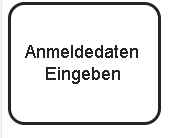
\includegraphics[scale=1.0]{Figures/Beispiel1}
\decoRule
\caption[Einfache Task]{Einfache Task - Anmeldedaten eingeben}
\label{Task}
\end{figure}Bei dem zweiten \textit{Leaf Block} handelt es sich nun um sogenannte \textit{Events}.Diese werden durch einen Kreis dargestellt uns anders als die Aufgaben passieren sie sofort. Es gibt unterschiedliche Typen, welche durch unterschiedliche Variationen eines Kreises dargestellt werden. Für uns relevant sind allerdings nur sogenannte \textit{catching Events}.  Erreicht der Token ein solches Event, wird gewartet bis das erwartete Ereignis auftritt und erst dann wird der Token weitergeschickt. Auch unter den catching Events gibt es drei grundsätzliche Unterscheidungen. Die einfachsten Variationen sind sogenannte \textit{Startevents}, welche einen Prozess Starten und durch einen einfachen dünn gezeichneten Kreis dargestellt werden und die \textit{Endevents}, welche den Prozess terminieren und durch einen einfachen dick gezeichneten Kreis dargestellt werden.\\
Durch die uns nun bekannten Bausteine, ist es uns möglich einen ersten Prozess aufzubauen und in BPMN zu Modellieren. In Abbildung \ref{ersterProz} sehen wir ein Beispiel für den ersten und einfachsten \textit{Nonleaf Block}. Den \textit{Prozess Block}. Dieser besteht aus einem Start- und einem Endevent. Zwischen den beiden Events liegt mindestens ein Task-Block und beliebig viele Event Blocks. Der Prozess in unserem Beispiel startet, indem ein Nutzer die Seite besucht und einen neuen Account anlegen möchte. Dieser wird zunächst auf eine Seite weitergeleitet, welche seine Anmeldedaten abfragt. Diese muss er dann in der ersten Aufgabe eingeben. Die zweite Aufgabe besteht nun darin den neuen Nutzer mit seinen eben angegebenen Daten in die vorhandene Datenbank einzutragen. Sobald diese Aufgabe erledigt ist, endet der Prozess und ein neuer Nutzer wurde erfolgreich angelegt.\\
\begin{figure}
\centering
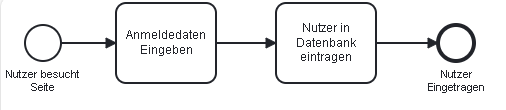
\includegraphics[scale=1.0]{Figures/Beispiel2}
\decoRule
\caption[Prozess Block]{Erster Vollständiger Prozessblock}
\label{ersterProz}
\end{figure}Events können allerdings auch während eines Prozesses auftreten. Wollen wir in unserem Beispiel einführen, dass die Startseite besucht werden kann, ohne, dass direkt auf die Nutzer anlegen Seite weitergeleitet wird, so können wir eine neue Aufgabe und ein fangendes Event einführen. Abbildung \ref{eventproz} zeigt diesen Prozess. Er startet, indem ein Nutzer die von uns erstellte Website besucht. Im nächsten Schritt wartet das catching Event, bis der Nutzer sich dazu entscheidet einen neuen Account anzulegen. In Folge dessen verhält sich der Prozess so, wie im Beispiel aus Abbildung \ref{ersterProz}. Events welche während dem Prozess auftreten werden \textit{Intermediate Events} genannt.
\begin{figure}
\centering
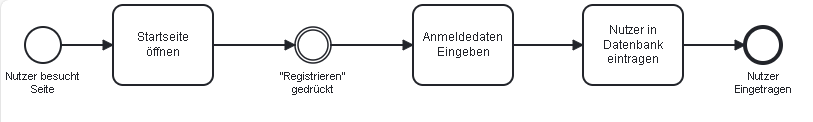
\includegraphics[scale=0.6]{Figures/Beispiel3}
\decoRule
\caption[Intermediate Events]{Beispiel für ein intermediate Event}
\label{eventproz}
\end{figure}
\subsection{Mögliche Verzweigungen}\label{Mögliche Verzweigungen}
In nun folgenden Abschnitt wollen wir uns mit Möglichkeiten beschäftigen den Sequenceflow zu verzweigen. Hierzu bietet BPMN einige sogenannte \textit{Gateways}. Um Gateways darzustellen, werden Rauten verwendet. Unterschiedliche Gateways haben unterschiedliche Symbole in den Rauten eingezeichnet. Sie sind dafür da, den Verlauf des Prozesses aufzuteilen und wieder korrekt zusammenzufügen. Wenn ein Gateway den Verlauf des Prozesses aufspaltet, so muss immer ein zweites Gateway den Verlauf wieder zusammenfügen. Eine Ausnahme hierfür wäre, wenn der Prozess in einer Verzweigung durch ein Endevent terminiert.\\
Um unser bislang erarbeitetes Beispiel etwas realitätsnaher zu gestalten, wollen wir eine neue Funktion einführen. Offensichtlich soll unsere Seite mehr Funktionen anbieten als neue Nutzer anzulegen. Die nächste logische Erweiterung ist eine Möglichkeit für bereits bestehende Kunden sich mit ihren vorhandenen Anmeldedaten einzuloggen. Hier spielt die erste Verzweigungsmöglichkeit eine Rolle. Da ein Nutzer immer entweder ein bestehendes Konto besitzt oder ein neues erstellen möchte, wird in jedem Durchlauf des Prozesses nur eine dieser Aktionen durchgeführt. Hier kann ein \textit{XOR-Gateway} genutzt werden. Es ist zu erkennen durch ein \textit{X} in der Raute. Es bietet die Möglichkeit zwischen unterschiedlichen Pfaden zu wählen. Im Beispiel aus Abbildung \ref{XOR} sehen wir eine mögliche Verwendung für dieses Gateway. Nachdem der Nutzer auf der Startseite den entsprechenden Button betätigt, wird er entweder zur Anmeldung oder zur Registrierung weitergeleitet. In beiden Fällen muss er seine Daten angeben. Je nachdem in welchem Teil wir uns befinden muss der Nutzer in der Datenbank eingetragen werden oder die Anmeldedaten müssen geprüft werden. Im Anschluss werden die zwei Äste wieder zusammengeführt und der Nutzer wird mit seinem zugehörigen Account auf der Seite angemeldet. Beim Zusammenführen der Äste, wartet das Gateway auf genau einen Token und gibt diesen dann weiter an das nächste Objekt. In diesem Beispiel ist der erste \textit{Flow Block} zu erkennen. Wird der Verlauf des Prozess durch ein XOR-Gateway aufgespalten und wieder zusammengeführt, so bilden alle Elemente innerhalb dieser Verzweigung im sogenannen \textit{Exclisive-choice-Block}. Abbildung \ref{XOR} zeigt außerdem eine Mögliche Variante des XOR-Gateways. Wenn der Nutzer einen vorhandenen Account anmelden möchte, aber inkorrekte Anmeldedaten eingibt, so wird er auf die Startseite zurückgeleitet. Das XOR-Gateway kann also auch für Loops verwendet werden. Hier ist zu erkennen, dass das zusammenführende Gateway durchaus auch vor dem aufspaltenden Gateway liegen kann. Es ist zusätzlich möglich auch mehr als zwei Ausgänge an das Gateway anzubinden.\\
\begin{figure}
\centering
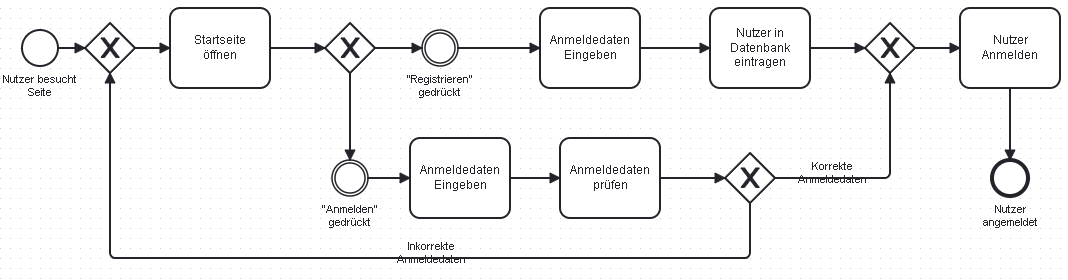
\includegraphics[scale=0.5]{Figures/Beispiel5}
\decoRule
\caption[XOR-Gateway]{Exclusive Entscheidung - Das XOR-Gateway}
\label{XOR}
\end{figure}Wir wollen nun ein weiteres Feature in unser Diagramm einfügen. Nachdem ein neuer Account erstellt wurde, soll dieser Nutzer nach wie vor angemeldet und auf die Homepage weitergeleitet werden. Zusätzlich soll er gleichzeitig auch für den Newsletter der Website eingetragen werden. Hierzu können wir ein weiteres Gateway nutzen. Das \textit{parallele Gateway} wird in Abbildung \ref{parallel} das erste Mal gezeigt. Es wird ebenfalls durch eine Raute dargestellt. Diese enthält allerdings ein \textit{+} in ihrem Inneren. An diesem Gateway wird der Verlauf des Prozesses wieder aufgespalten. Anstelle von nur einem Strang werden hier aber alle Gelichzeitig ausgeführt. Das zusammenführende Gateway muss desshalb nicht blind den ersten Token weiterschicken, den es erhält, sondern wartet bis an allen Eingängen ein Token vorliegt, fügt diese wieder zusammen und gibt dann den Token weiter an das nächste Objekt. Hier können Schwierigkeiten auftreten, falls ein paralleler Zweig in einem Endevent endet. Bei der Modellierung eines Diagrammes muss dies also verhindert werden. Insgesamt spricht man hier von einem \textit{Parallel Block.}\\
\begin{figure}
\centering
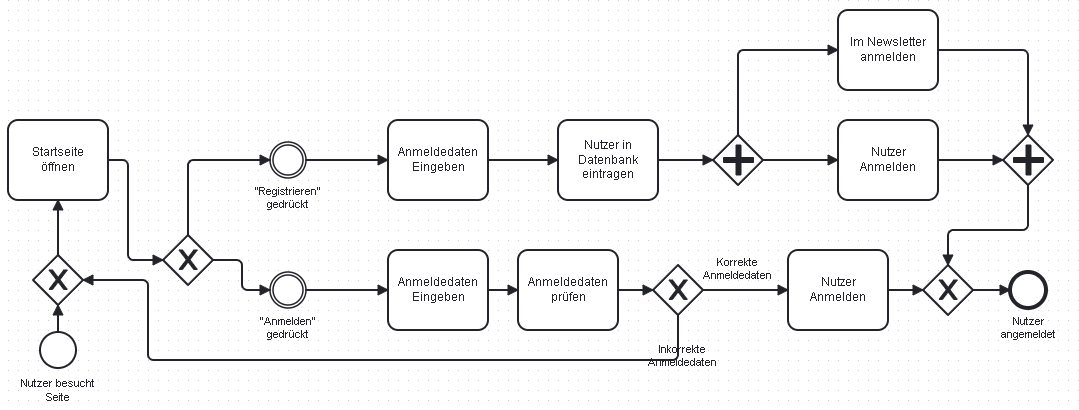
\includegraphics[scale=0.5]{Figures/Beispiel6}
\decoRule
\caption[Paralell-Gateway]{Parallele Ausführung - Das Paralell-Gateway}
\label{parallel}
\end{figure}
\subsection{Subprozesse und weitere Elemente}\label{Subprozesse und weitere Elemente}
Der letzte Block, welcher von uns genauer betrachtet wird ist der \textit{subprocess-Block}. Auch dieser wird bereits durch den Namen gut beschrieben. Zur vereinfachten Darstellung, kann ein Teil von einem Prozess als ein unterprozess zusammengefasst werden. In Abbildung \ref{subprozess} ist also der selbe Prozess dargestellt wie der in Abbildung 2.5. Hier wurde der Teil des Prozesses, in dem ein Nutzer registriert wird zu einem Subprocess zusammengefasst. In Abbildung \ref{alleElem} findet sich zudem eine Alternative Darstellung dieses Blockes. Hier ist zu sehen, dass der Subprozess auch als einzelnes Elemt auftauchen kann. An der Stelle wird dann eine referenz zu einem Prozess gemacht. Dieser enthält die Elemente die von dem Subprocess ausgeführt werden. In dieser Abbildung ist zustätzlich noch eine Übersicht über alle für uns relevante Elemente zu finden.\\
\begin{figure}
\centering
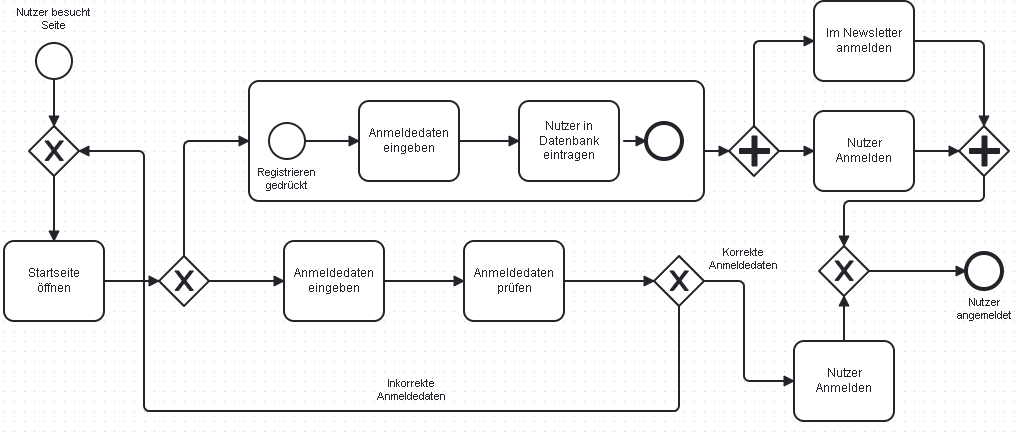
\includegraphics[scale=0.5]{Figures/Beispiel7}
\decoRule
\caption[Subprocess Block]{Subprocess Block - Prozesse innerhalb von Prozessen}
\label{subprozess}
\end{figure}Zuletzt möchten wir nun jene Elemente beschreieben, die für unsere Arbeit nicht wichtig werden. Hierbei handelt es sich zum großteil um Varianten der uns bekannten Bausteine. Neben den Exclusive und Parallel Gateways existieren noch sogenannte \textit{Event-based Gateways}. Diese entscheiden anhand eines eintreffenden Events, wleche Aktion ausgefürt wird. 
Die Task blocks lassen sich durch Symbole in der oberen linken Ecke genauer spezifizieren. Hier wird unterschieden zwischen \textit{User task, Service task, Business rule task} und \textit{Script task}. Auch unter den Events kann genauer spezifiziert werden. Für alle \textit{catching events} sind \textit{throwing events} vorhanden und auch unter diesen gibt es unterschieldiche Typen wie \textit{Message Evens} oder \textit{timer Events}. Zudem gibt es eine Möglichkeit Datenflüsse darzustellen durch eine sogenannte \textit{Date object reference} oder eine \textit{Data store reference}. Zuletzt bietet BPMN eine möglichkeit verschiedene Teilnehmer einer Prozesses darzustellen. Sogenannte \textit{pools} und \textit{lanes} können genutzt werden um Gruppen und auch einzenle Teilnehmer innerhalb dieser Gruppen darzustellen.\\
\begin{figure}
\centering
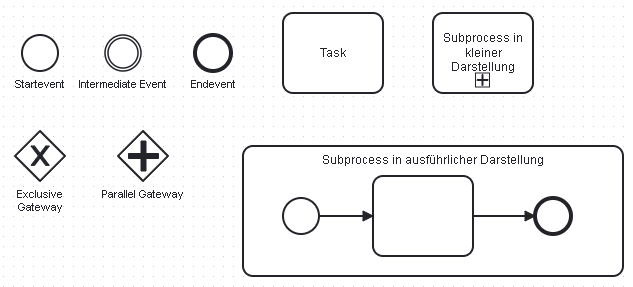
\includegraphics[scale=0.5]{Figures/Alleblocke}
\decoRule
\caption[Alle Elemente]{Alle von uns genutzten Elemente}
\label{alleElem}
\end{figure}
\section {Prozessalgebra - ACP}\label {Prozessalgebra - ACP}
Nachdem wir die wichtigsten Bestandteile der Modellierungssprache BPMN eingeführt haben, wollen wir uns nun mit der Prozessalgebra ACP (Algebra of Communicating Processes) beschäftigen und diese mit ihren einzelnen Bestandteilen genauer erläutern.\\
Parallel zu den Tasks in BPMN sprechen wir hier von sogenannten \textit{Aktionen}. Diese werden klein geschrieben und können ansonsten beliebig benannt werden. Auch Prozesse und Sub-prozesse werden hier angewendet. Die Syntax für einen Prozess welcher eine beliebige Aktion ausführt ist durch P::=v gegeben. Ein mögliches Beispiel ist auch hier wieder das Registrieren eines neuen Nutzers. P::=nutzerRegistrieren beschreibt also den Prozess P welcher die Aktion nutzerRegistrieren ausführt. Analog dazu können auch Subprozesse dargestellt werden. P::=K beschreibt den Prozess P welcher daraus besteht die Prozess K auszuführen. Dies kann zur vereinfachten Darstellung von ausführlicheren Prozessen oder zur Darstellung von Rekursion genutzt werden.\\
Ähnlich wie bei BPMN können Prozesse und Aktionen in ACP konkateniert werden. Hierzu wird der *-Operator verwendet. Der Prozess, welcher im Beispiel aus Abbildung \ref{ersterProz} als BPMN Diagramm dargestellt ist, kann also durch P::=nutzerBesuchtSeite*anmeldedatenEingeben*nutzerInDbEintragen*nutzerEingetragen in ACP dargestellt werden.\\
Für die Gateways, welche in Abschnitt \ref{BPMN} erläutert wurden, gibt es auch in ACP Darstellungsmöglichkeiten. Zunächst wollen wir die XOR-verknüpfung erklären. Diese wird durch den +-Operator dargestellt. Auch hier kann ein zuvor durch BPMN modelliertes Beispiel verwendet werden. Wir können hierzu das in Abbildung \ref{XOR} gezeigte Diagramm in eine Formel in ACP umwandeln. Zur vereinfachten Darstellung wollen wir folgende Abkürzungen verwenden.\\
sO -> Startseite Öffnen\\
aE ->Anmeldedaten Eingeben\\
nE ->Nutzer Eintragen (In DB)\\
aP ->Anmeldedaten Prüfen\\
nA ->Nutzer Anmelden\\
Eine mögliche lösung könnte wie folgendermaßen aussehen.\\
P::=sO*((aE*nE)+(aE*aP))*nA\\
Die Klammern können so interpretiert werden, dass die umschlossenen Terme zusammenhängen. Es wird in dem Beispiel also entweder (aE*nE) oder (aE*aP) ausgeführt.\\
Als nächstes wollen wir nun veranschaulichen wie das Parallel-Gateway aus BPMN in APC umgesetzt wird. Hierzu gibt es drei unterschiedliche sogenannte \textit{Merge Operatoren}. Diese sollen hier nun einzeln erklären.
Zunächst betrachten wir den \textit{regulären Merge Operator}. Dieser wird durch ein || dargestellt und beschreibt das parallele Ausführen zweier Prozesse. Sollte der Prozess P also durch P::=Q||R beschrieben werden, so ist egal welcher der beiden Subprozesse Q oder R zuerst eine Aktion ausführt.\\
Als nächstes beschreiben wir nun den \textit{Left Merge Operator}. Dieser wird durch ein $\leftMerge$ dargestellt. Auch hier werden beide Subprozesse ausgeführt. Es muss allerding zuerst der Linke der beiden eine Aktion ausführen. Im Anschluss verhält sich der Operator genauso wie der reguläre Merge-Operator. Zuletzt betrachten wir den \textit{Communication Merge Operator}, welcher durch ein | dargestellt wird. Hier werden beide Subprozesse gleichzeitig in einem Schritt ausgeführt.
\section{Datenbanken}\label{Datenbanken}
Im folgenden Kapitel werden nun Relationale Datenbanken genauer beschrieben. Wir betrachten zunächst ein Relationsschema  $\mathcal{R} = \{R_1/a_1,…,R_n/a_n\}$. Dies beinhaltet eine Menge an Relationen $R_i$, welche jeweils eine zugehörige Stelligkeit $a_1$ besitzen. Dieses Schema beschreibt unsere Datenbank. Jede Relation $R_i$ aus  $\mathcal{R}$ kann als Tabelle der Datenbank angesehen werden. \\
Auch hier findet das in den Vorherigen Abschnitten verwendete Beispiel Anwendung. Um den Registrierungs- und Anmeldeprozess umsetzen zu können, müssen zumindest die Kontodaten jedes Nutzers gespeichert werden. Diese beinhalten in unserem Beispiel lediglich den Nutzernamen und das Passwort. Unser Beispiel benötigt also nur eine Tabelle. Das bedeutet, dass in unserem Relationsschema nur eine Relation hinterlegt ist. Diese könnte beispielsweise den Namen Nutzer tragen. Da die Tabelle Nutzer aus den zwei Spalten Nutzername und Passwort besteht beträgt die Stelligkeit der Relation zwei. Das Relationsschema aus unserem Beispiel lautet also $\mathcal{R}_1=\{Nutzer/2\}$. \\
Zusätzlich definieren wir den Begriff der Domäne ${\Delta}$ einer Datenbank als jene zählbar unendliche Menge, welche sämtliche Datentypen enthält, die in der jeweiligen Datenbank vorkommen können. Sie beschränkt sich in unserem Beispiel also auf alle Strings. \\
Eine Instanz $\mathcal{I}$ einer Datenbank ist ebenfalls als eine Menge zu betrachten. Diese Menge enthält sämtliche Daten, die zu einem gewissen Zeitpunkt in der Datenbank abgespeichert werden. Diese Daten werden in Form von Tupeln abgespeichert. Ein Tupel enthält jeweils den Namen der jeweiligen Relation, sowie die Daten eines Elements. Auch hier dient das oben bereits verwendete Beispiel gut zu Veranschaulichung. Befindet beispielsweise ein Nutzer mit dem Nutzernamen \textit{Marin} und dem Passwort \textit{Test} in der Datenbank, so ist $\mathcal{I}_1 = \{(Nutzer, Marin, Test)\}$. Wird nun ein weiterer Nutzer mit dem Nutzernamen \textit{Max} und dem Passwort \textit{pw} hinzugefügt, so wird $\mathcal{I}$ um das Tupel (Nutzer, Max, pw) erweitert. Also ist $\mathcal{I}_2 =\{(Nutzer, Marin, Test), (Nutzer, Max, pw)\}$. Eine Alternative Schreibweise ist durch $\mathcal{I}_2 = \{Nutzer(Marin, Test), Nutzer(Max, pw)\}$ gegeben. Der Name der Relation kann also auch außerhalb der Klammern stehen.\\
In Abbildung 2.8 ist zur veranschaulichung eine Tabelle zu sehen, welche die Inhalte von $\mathcal{I}_2$ überscihtlicher darstellen soll.\\
\begin{figure}
\centering
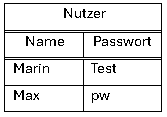
\includegraphics[scale=1]{Figures/Tabelle1}
\decoRule
\caption[Tabelle1]{$\mathcal{I}_2$ graphisch dargestellt}
\label{fig:Task}
\end{figure}Wollen wir die Datenbank nun um eine Weitere Tabelle erweitern, welche beispielsweise zwei Nutzer durch eine Freundschaft verknüpft und zusätzlich speichert seit wie vielen Jahren diese Freundschaft besteht, so wird kann das gegebene Schema $\mathcal{R}_1$ um \textit{Freuzndschaft/3} erweitert werden. Also $\mathcal{R}_2=\{Nutzer/2, Freundschaft/3\}$ dei drei Attribute der Relation Freundschaft sind hierbei Freund\_1, Freund\_2 und Dauer. Das Attribut Dauer beschreibt seit wie vielen Jahren eine Freundschaft besteht und wird als Integer angegeben. Durch diese Änderung wird die Domäne ${\Delta}$ zusätzlich um sämtliche Integer erweitert. 
Fügen wir nun eine Freundschaft zwischen \textit{Max} und \textit{Marin}, welche seit 0 Jahren besteht der Datenbank hinzu, so wird  $\mathcal{I}$ um das Tupel (Freundschaft, Max, Marin, 0) erweitert. Also $\mathcal{I}_3$= \{Nutzer(Marin, Test), Nutzer(Max, pw),Freundschaft(Max, Marin, 0)\}. Abbildung 2.9 zeigt die Instanz in Form von Tabellen.\\
\begin{figure}
\centering
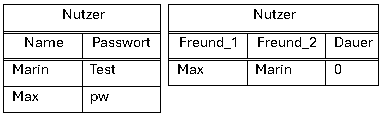
\includegraphics[scale=1]{Figures/Tabelle2}
\decoRule
\caption[Tabelle2]{$\mathcal{I}_3$ graphisch dargestellt}
\label{fig:Task}
\end{figure}Das sogenannte  \textit{Universum} enthält alle möglichen Instanzen in Bezug auf das Schema und der Domäne. $\mathcal{I}_1$, $\mathcal{I}_2$ und $\mathcal{I}_3$ sind also Elemente des Universums.\\
Nun wollen wir betrachten, wie Datenbanken manipuliert werden können.\\
Hierzu müssen wir zunächst betrachten, wie Daten aus der Datenbank ausgelesen werden können.\\
Dazu nutzen wir sogenannte Queries. Diese werden in FOL ausgedrückt. Hierzu definieren wir zunächst eine Menge $VARS = \{u_1,…,u_n\}$. Diese Menge besteht aus Variablen, welche alle Werte aus ${\Delta}$ annehmen können. Zusätzlich bildet eine Substitution ${\sigma}$ alle Variablen auf Vars auf werte in ${\Delta}$ ab. \\
 Eine Query ${\phi}$ ist durch folgende Syntax gegeben: \\
${\phi}$ ::= true | R($u_1$, . . . , $u_a$) | ${\neg}{\phi}$ | ${\phi}_1$ $\wedge$ ${\phi}_2$ | $\exists$u.${\phi}$ | $u_1$ = $u_2$ \\
Wir wollen nun die Semantik dahinter erläutern.
\begin{itemize}
\item Für ${\phi}$ ::= true besteht die Query in jedem Fall.
\item Für ${\phi}$ ::= R($u_1$, . . . , $u_a$) besteht die Query, falls das Tupel R($e_1$, … ,$e_a$) in I vorliegt. Hierbei ist $e_i$=${\sigma}$($u_i$) für alle i: 1 </= i </= a.
\item Für ${\phi}$ ::=${\neg}$ Q besteht die Query, falls Q nicht bestehen würde. 
\item Für ${\phi}$ ::= Q1 $\wedge$ Q2 besteht die Query, wenn Q1 und Q2  bestehen würden
\item Für ${\phi}$ ::= $u_1$ = $u_2$  besteht die Query, wenn ${\sigma}$($u_1$)=${\sigma}$($u_2$)
\item Für ${\phi}$::= $\exists$u.Q besteht die Query, wenn in der aktuellen Instanz der Datenbank ein Element existiret, welches durch eine Substitution  ${\sigma}$' auf u abgebildet werden kann. 
\end{itemize}
Die Manipulation einer Datenbank besteht aus drei Phasen. Zunächst muss ein eine Query, welche wir als Guard bezeichnen bestehen. Im Anschluss kann die Aktion ausgeführt werden. Die Aktion besteht aus dem löschen eines Elements und dem Hinzufügen eines Elements. Ein Element beschreibt dabei ein Tupel in der Menge $\mathcal{I}$ Hier ist anzumerken, dass es keine Möglichkeit gibt Inhalte der Datenbank zu ändern. Möchte also ein Nutzer sein Passwort ändern, so wird zuerst in einem Schritt der jeweilige Nutzer entfernt und im nächsten Schritt ein neuer Nutzer mit dem veränderten Passwort der Datenbank hinzugefügt.









